Wearable health monitoring devices have been progressing in areas including
form factor, biometric data collection, and battery life.  This section will
discuss the current state of commercially available solutions, as well as some
ongoing research areas.

Commercially available wearable health monitoring devices come in a variety of
different form factors depending on their intended use and their capabilities.
These include wrist-mounted devices such as smartwatches and wrist bands,
head-mounted devices, straps, textiles, and various
others \cite{Seneviratne2017}.  The type of device most relevant to this
proposal is the wrist band.  They may be equipped with a selection of sensors
and a processor, but have no display.  An example of such a device shown in 
Figure \ref{fig:EmpaticaE4} is the Empatica E4 wristband \cite{McCarthy2016}.  
This device is designed to provide real-time
physiological data for research using a photoplethysmogram, electrodermal
activity sensor, accelerometer, and temperature sensor \cite{empatica}. The
device can log data internally, stream it over Bluetooth, and has an API for
developing smartphone apps that make use of the data it collects. Empatica
claims that their device has been used by researchers in over 1000 studies
\cite{empatica}.

\begin{figure}[!htb]
\centering
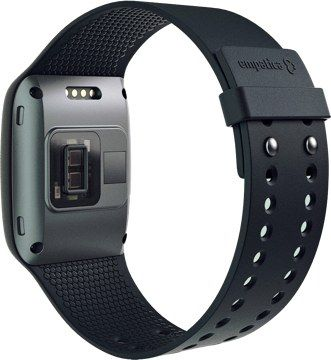
\includegraphics[scale = 0.5]{images/EmpaticaE4.jpg}
\caption{Empatica E4 wristband. Reproduced from \cite{empatica}.}
\label{fig:EmpaticaE4}
\end{figure}

Many modern wearable health monitoring devices offer a similar suite of sensors
that measure heart rate, temperature, motion, and more
\cite{Seneviratne2017}.  A novel type of sensor that has yet to be incorporated
into these devices is a sweat sensor.  Sweat sensors are chemical sensors that
can non-invasively analyze the user's sweat at a molecular level in order to
detect biomarkers \cite{Tai2018}.  If sweat is not produced naturally, the 
sensors can induce sweating to facilitate measurements \cite{Tai2018}.  One of 
the limitations on the number and type of sensors that can be put in a wearable 
device is their location, since some sensors require specific placement on the
body \cite{Baig2017}.  A workaround for this problem is to use textile sensors 
\cite{Hatamie2020}.  If the wearable device is a pair of socks for example, 
then several pressure sensors can be placed under the pressure points of the 
users foot in order to provide useful information to athletes \cite{Hatamie2020}.
It is easy to imagine how this can be extended to other types of garments as well
to provide much more freedom in sensor placement than what is allowed by something 
like a wrist band.  Nanomaterial sensors are being developed that can be placed either directly 
on skin or made into textiles that can be worn \cite{Yai2018}.  Many sensors can 
be made using this technology including temperature sensors, strain rate sensors, 
tactile sensors, electrophysiological sensors, electrochemical sensors, and more 
\cite{Yai2018}.

Like smart-phones or other mobile devices, powering wearable health monitoring
devices can be a challenge \cite{Pantelopoulos2010}.  Longer battery life is 
desirable but usually comes at the cost of weight and size.  
Wearable devices place yet another constraint on this problem: comfort 
\cite{Motti2014}.  Greater levels of comfort allow users to wear the device 
continuously for long periods of time \cite{Motti2014}.  

One way of overcoming the battery problem is through the use of specialized 
textiles that can generate or store electricity.  Triboelectric 
nanogenerator fabric can be used to generate electricity from the movement of 
the person wearing it, and that energy can be stored in another fabric which 
is made with supercapacitor yarn \cite{Pu2016}. An example of how these fabrics 
may be integrated into clothing and arranged on a persons body can be seen in 
Figure \ref{fig:EnergyFabric}.  The energy produced by these fabrics can then 
be used to power the electronics of the wearable device \cite{Pu2016}.  Another 
method of generating electricity from the wearer of the device is to take 
advantage of body heat \cite{Siddique2017}. This can be done using wearable 
thermoelectric power generators that are flexible and conform to the area of the 
body they are attached to \cite{Siddique2017}.  They rely on a temperature 
difference between the ambient air and the surface they are attached to in order 
to generate electricity \cite{Siddique2017}.  Wearable devices that rely on 
batteries can also take advantage of specialized textiles.  Zinc ion batteries 
have been made into film that is both flexible and safe in the case of impact, 
puncture, and washing \cite{Li2018}.

\begin{figure}[!htb]
\centering
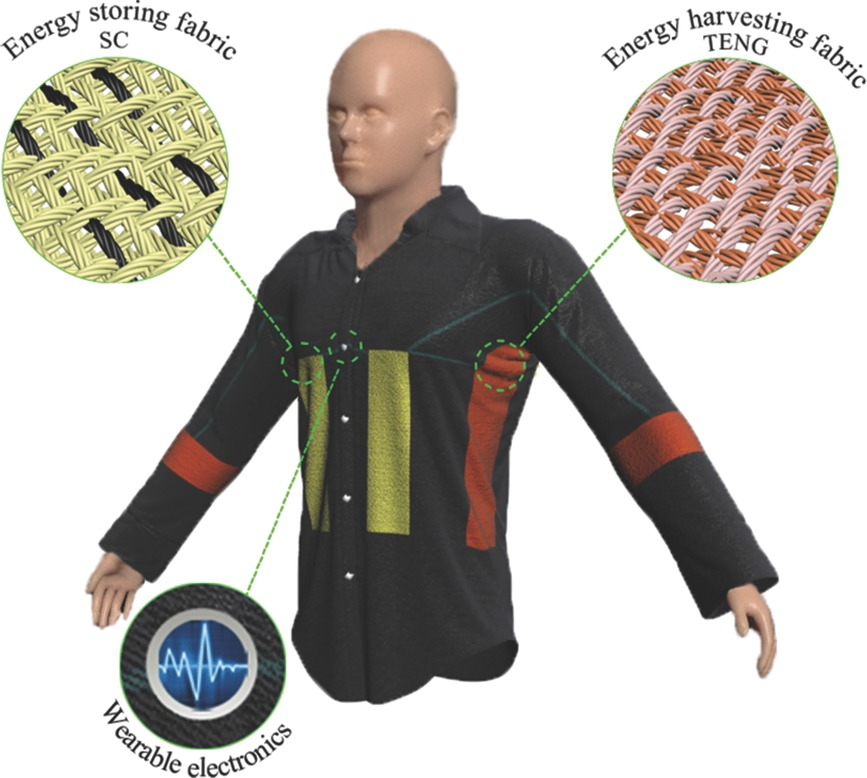
\includegraphics[scale = 6]{images/EnergyFabric.jpg}
\caption{Energy generation and storage textile. Reproduced from \cite{Pu2016}.}
\label{fig:EnergyFabric}
\end{figure}

A contrasting approach to reducing the battery capacity requirement of wearable 
devices is power conservation.  Dynamic power consumption of electronic 
components is related to their supply voltage, capacitance, and operating 
frequency \cite{Forman1994}. All three of these factors can be reduced in order 
to save power.  Supply voltage can be reduced by using components designed to 
operate on lower voltages, capacitance can be reduced by using highly integrated 
components or multichip modules, and frequency can be reduced by lowering 
processor clock speeds at the cost of performance \cite{Forman1994}.  
Technologies like Wafer Level Fan Out System-in-Package are contributing to 
higher levels of electronic integration by combining active components and 
passive components into a single package \cite{Martins2018}. Not only does this 
aid in lowering power consumption, but helps miniaturize wearable devices as 
well \cite{Martins2018}.
An embedded processor in a wearable device could make 
use of an adjustable clock, or multiple clock sources in order to slow the 
processor down when high performance is not needed and conserve power.  This 
technique coupled with others like dynamic voltage scaling have proven 
useful to help energy harvesting IoT devices make the best use of fluctuating
and intermittent power sources \cite{Ma2017}.
Even when high performance is needed certain tasks can be offloaded to dedicated
hardware that is more efficient, thus allowing the processor to remain in a 
lower power state.  AES encryption for example has been shown to have lower 
power consumption and increased performance when dedicated hardware is used
instead of a software implementation \cite{Hamalainen2006}.  For this reason,
wearable devices using encryption for communication or data storage may 
benefit from using a processor with hardware cryptography support. Another task
directly related to wearable devices that has seen benefit from hardware 
acceleration is real time ECG signal processing \cite{Cardarilli2018}. It was 
shown that hardware acceleration allowed for a reduction in processor clock 
speed without sacrificing execution time, resulting in significant power 
savings.

By combining the power generation, storage, and conservation technologies 
aforementioned, it may be possible to create future wearable health monitoring 
devices that are just as comfortable to wear as regular clothing, never 
require charging, and are essentially maintenance-free for the life of the unit.

In summary, it appears that significant research and development has gone into
moving wearable health monitoring devices away from the current design of a
battery-powered device affixed to the body in some way, and towards comfortable
textiles that cover the body, monitor biometrics, and power themselves from the
body.  Unfortunately, the technology required for these desirable qualities is 
not yet mature enough to be inexpensive and readily available to use in this this project.  
As a result, the wearable device this project aims to create will have to be 
more in line with some of the commercially available products out there today. 
It is possible however to apply some of the power conservation techniques using 
technology available today. Hardware acceleration and higher levels of 
integration can be achieved using embedded processors with several built in
modules for things like Bluetooth, USB, cryptography, and more. An example of
such a processor is the nRf52840 made by Nordic Semiconductor. There are also
sensors available that integrate measurement of several different parameters 
and may even perform some signal processing all in a single chip such as the 
TDK InvenSense ICM-20948 inertial measurement unit. Many opportunities exist 
for a wearable device to slow down or stop its processor in order to save power, 
such as between sensor readings, or when not interacting with the user. All of 
these technologies, constraints and possibilities are important considerations 
when designing a wearable health monitoring device.
